%---------------------------------------------------------------------------------------------------
% Routing-Atlas
%---------------------------------------------------------------------------------------------------
\section{Routing-Atlas}\label{sec:routingatlas}


Der Routing-Atlas~\cite{wsbh-envgi-12} ist ein Projekt der inet-AG in Zusammenarbeit mit dem BSI.
Ziel ist die Untersuchung der Topologie des Internets auf AS-Ebene.
Gegenüber vorherigen Ansätzen wurde hierbei ein besonderer Fokus auf die die Kriterien Staat und Branche gelegt.
Dabei sollte geklärt werden, in wie weit eine nationale Klassifizierung des Internets auf IP- und AS-Ebene möglich ist, in wie weit das Routing einer Nation in sich abgeschlossen ist und wie starke Abhängigkeiten bestehen.

Das Routing-Atlas Projekt nutzt verschiedene Datenquellen und führt diese zusammen.
\begin{itemize}
  \item Informationen zu IP-Adressblöcken und -Präfixen sowie zu ASen aus der RIPE-Datenbank~\cite{ripe-db} und vom Team Cymru~\cite{cymru}
  \item Datensätze regionaler Monitore~\cite{ripe-ris}
  \item Matrizen zu Shortest Path und Next Hop des NEC labs, die Rolf Winter erstellt hat~\cite{neclab-topology, Winter:2009:MIR:1577959.1577976}
  \item Hierarchische Einordnung der ASe auf Basis von Daten, die von einer Arbeitsgruppe der UCLA um Lixia Zhang gesammelt werden~\cite{ucla-topology, Zhang:2005:CIA:1052812.1052825}
\end{itemize}

%
Die Toolchain des Routing-Atlas besteht aus den vier Schritten Identifizieren, Aggregieren, Klassifizieren und Visualisieren.

Identifiziert werden zunächst alle IP-Adressblöcke in der RIPE Datenbank, die eine Länderkennung \emph{DE} oder \emph{EU} tragen.
Für die lediglich als europäischen Ursprungs gekennzeichneten Adressblöcke wird über administrative Adressen versucht eine nähere Einordnung vorzunehmen.
Hieraus resultiert die Menge aller deutschen IP-Adressblöcke.

Die so ausgewählten Adressblöcke zu IP-Präfixen aufgelöst.
Im folgenden Schritt werden die Präfixe den jeweiligen Autonomen Systemen zugeordnet.
Hierzu werden (in dieser Reihenfolge) die RIPE DB, die Datenbank des Team Cymru und ein Route-Monitor verwendet.
Das Resultat ist die Menge aller Autonomen Systeme die einen deutschen IP-Adressblock besitzen.

Die Autonomen Systeme werden nach zwei Kriterien klassifiziert.
Zum einen wird eine hierarchische Einordnung vorgenommen.
Zum anderen werden die ASe Branchen zugeordnet.

Die Hierarchie eines Autonomen Systems wird aus der „Internet Topology Collection“ der UCLA übernommen~\cite{ucla-topology}.
Basierend auf ihrem Knotengrad und der Art der Verknüpfung untereinander werden die ASe eingeordnet in:
\begin{itemize}
  \item Tier-1: AS hat keine Provider
  \item Large ISP: AS ist Provider für mehr als 50 Kunden
  \item Small ISP: AS hat zwischen 5 und 50 Kunden
  \item Stub: AS hat weniger als 5 Kunden
\end{itemize}
Die Position eines AS in der Hierarchie wird später bei der Visualisierung benötigt.

Die Klassifizierung der Autonomen Systeme in Branchen erfolgt anhand von Schlüsselworten nach denen in gesammelte Informationen, Namen und Adressen gesucht wird.
Die Zuordnung eines AS zu einer Branche ermöglicht den Vergleich verschiedener Branchenspezifischer Netzabschnitte oder beispielsweise die Analyse der Konnektivität zweier Branchen untereinander.

Für die Visualisierung werden Teilgraphen gebildet und auf verschiedene Weise dargestellt.
Die Teilgraphen behinhalten dabei alle oder eine nach beispielsweise einer Branche gefilterte Teilmenge der deutschen Autonomen System sowie alle verbindende ASe.
Die verbindenden ASe sowie die Pfade werden aus den Matrizen von Winter~\cite{Winter:2009:MIR:1577959.1577976} extrahiert.

\begin{figure}
  \begin{center}
    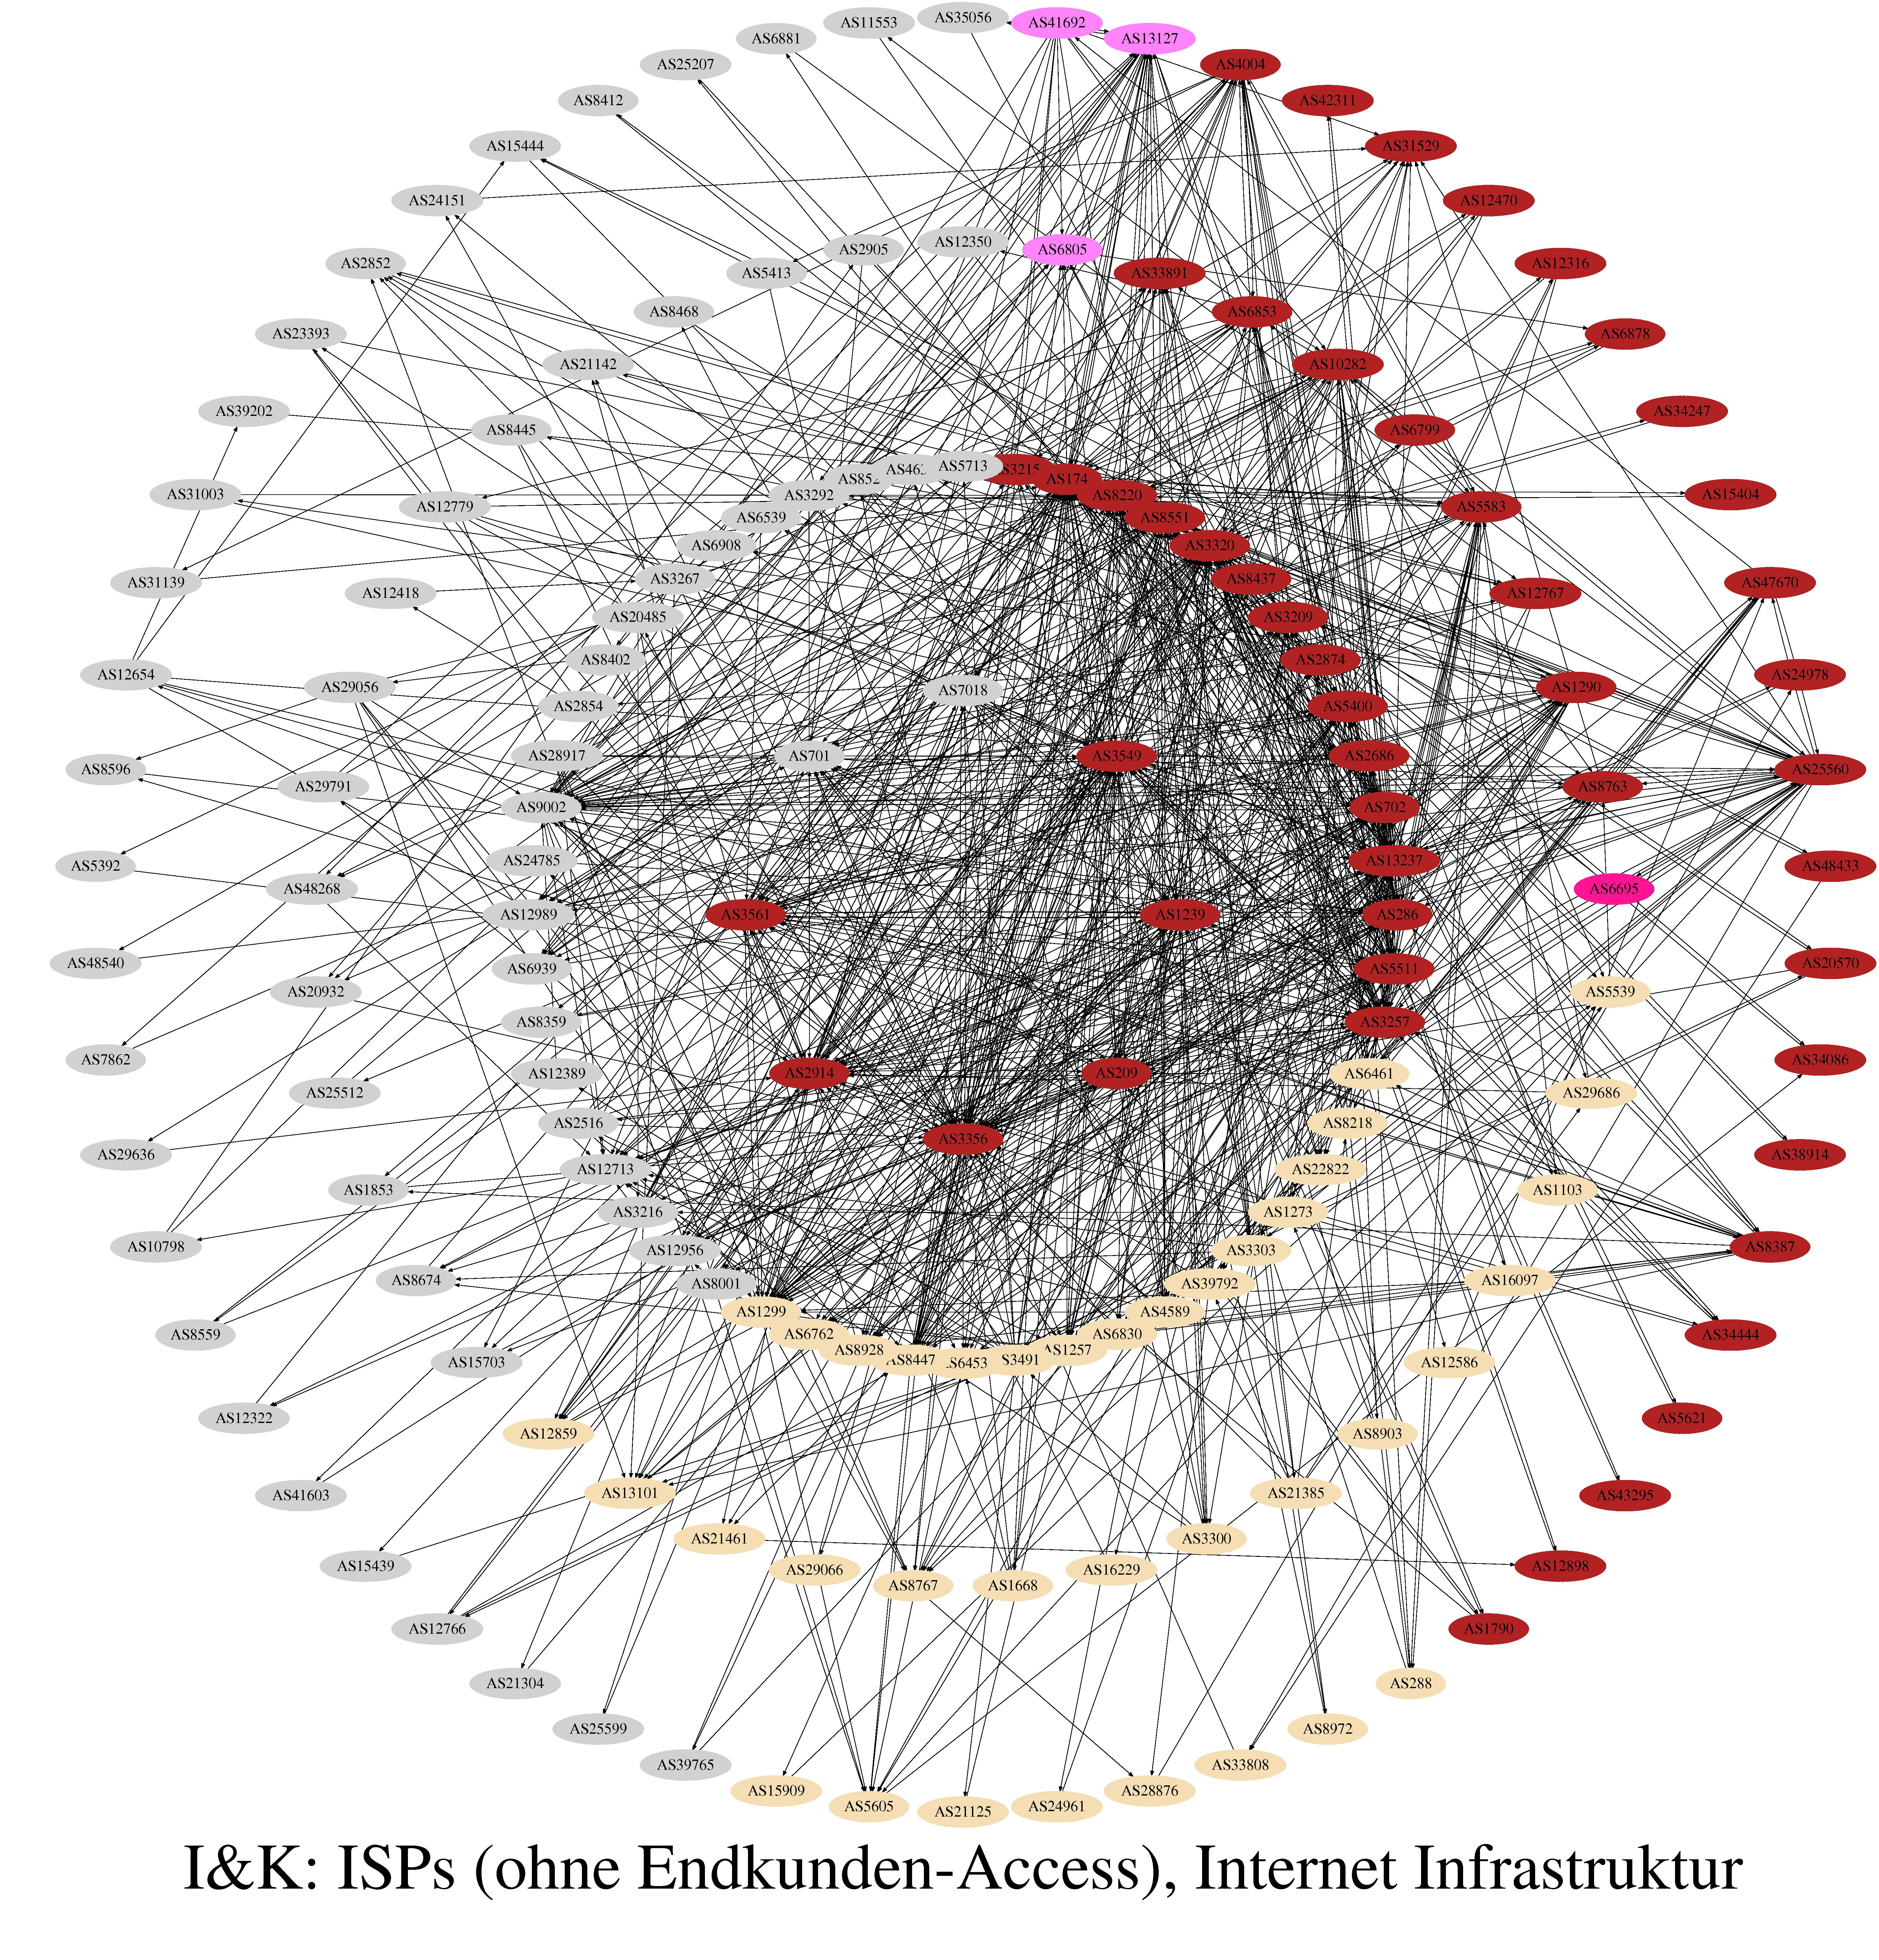
\includegraphics[width=.8\textwidth]{asgraph_cat4-pos}
    \caption{Hierarchisches Kreismodell - Entnommen aus~\cite{swbh-rsved-11}} \label{asgraph}
  \end{center}
\end{figure}

Der Graph in Abb.~\ref{asgraph} zeigt beispielsweise die Autonomen Systeme der Branche ISPs (ohne Endkunden-Access) und Internet Infrastruktur sowie deren verbindende ASe.
Von innen nach außen entspricht dabei die Anordnung der hierarchischen Klassifizierung von Tier-1 bis Stub.
